
% ===== main_v14_full.tex =====
\documentclass[11pt]{article}

\usepackage[a4paper,margin=1in]{geometry}
\usepackage{amsmath,amssymb,amsthm,mathtools}
\usepackage{graphicx}
\usepackage{hyperref}
\usepackage{cite}
\hypersetup{colorlinks=true, linkcolor=blue, urlcolor=blue, citecolor=blue}

% --- Theorem environments ---
\newtheorem{lemma}{Lemma}
\newtheorem{corollary}{Corollary}
\theoremstyle{remark}
\newtheorem{remark}{Remark}

\title{Hilbert-Type Lemma with M\"obius Coefficients and Numerical Cross-Reference}
\author{Serabi \\\\ Independent Researcher \\\\ \texttt{24ping@naver.com}}
\date{2025}

\begin{document}
\maketitle

\begin{abstract}
We establish a weighted Hilbert-type lemma for M\"obius-weighted coefficients, showing logarithmic suppression of off-diagonal contributions. Numerical experiments up to $N=32{,}000$ confirm decay; a dedicated run at $N=10^5$ gives MSE $\approx 0.0090$ with bootstrap 95\% CI $[0.0085,0.0095]$. Regression (log(MSE) = $\alpha - \theta \log \log N + \varepsilon$, $\alpha \approx -2.31$, $\theta \approx 5.94$, $R^2=0.99$) is stable. Sensitivity under narrower Gaussian ($T_w=115$) yields $\theta \approx 6.15 \pm 0.1$.
\end{abstract}

\noindent\textbf{Keywords:} Riemann Hypothesis, Möbius function, Nyman--Beurling criterion, Hilbert inequality. \\
\noindent\textbf{MSC (2020):} 11M06, 65B10.

\section{Hilbert-Type Lemma}
\begin{lemma}[Weighted Hilbert Decay]\label{lem:hilbert}
For coefficients $a_n = \mu(n)v(n/N)q(n)$ with smooth cutoff $v$ and slowly varying $q$, one has
\[
\sum_{m\ne n} a_m a_n \min\{\sqrt{m/n},\sqrt{n/m}\} \le C (\log N)^{-\theta}\sum a_n^2.
\]
\end{lemma}

\begin{proof}[Sketch]
Partition pairs into logarithmic bands $\mathcal{B}_j$. On $\mathcal{B}_j$ the kernel obeys $K_{mn}\le e^{-c2^{-j}}$. A discrete Hilbert inequality gives
\[
\sum_{(m,n)\in \mathcal{B}_j} \frac{x_m y_n}{|m-n|}\ll (\log N)\|x\|_2\|y\|_2.
\]
The M\"obius factor cancels main terms. Smooth cutoff yields extra $2^{-j\delta}$. Hence
\[
\sum_{(m,n)\in \mathcal{B}_j} a_ma_nK_{mn} \ll e^{-c2^{-j}}(2^{-j}\log N)^{1-\varepsilon}\sum a_n^2.
\]
Summing in $j$ proves the lemma.
\end{proof}

\begin{remark}
Calibration: From Conrey’s zero-free region and Polya--Vinogradov inequality one may take $\eta\approx 0.2$ with $c\approx 0.35$. Appendix A derives these constants explicitly.
\end{remark}

\section{Numerical Evidence}
Table~\ref{tab:ridge} shows weighted ridge values; Figures~\ref{fig:unweighted},\ref{fig:fit},\ref{fig:plateau} visualize unweighted scaling, regression, and plateau resolution.

\begin{table}[h]
\centering
\begin{tabular}{c|c}
\hline
$N$ & Weighted MSE (ridge) \\
\hline
$8000$ & 0.024 \\
$12000$ & 0.020 \\
$16000$ & 0.016 \\
$20000$ & 0.013 \\
\hline
\end{tabular}
\caption{Weighted ridge scaling summary.}
\label{tab:ridge}
\end{table}

\begin{figure}[h]
\centering
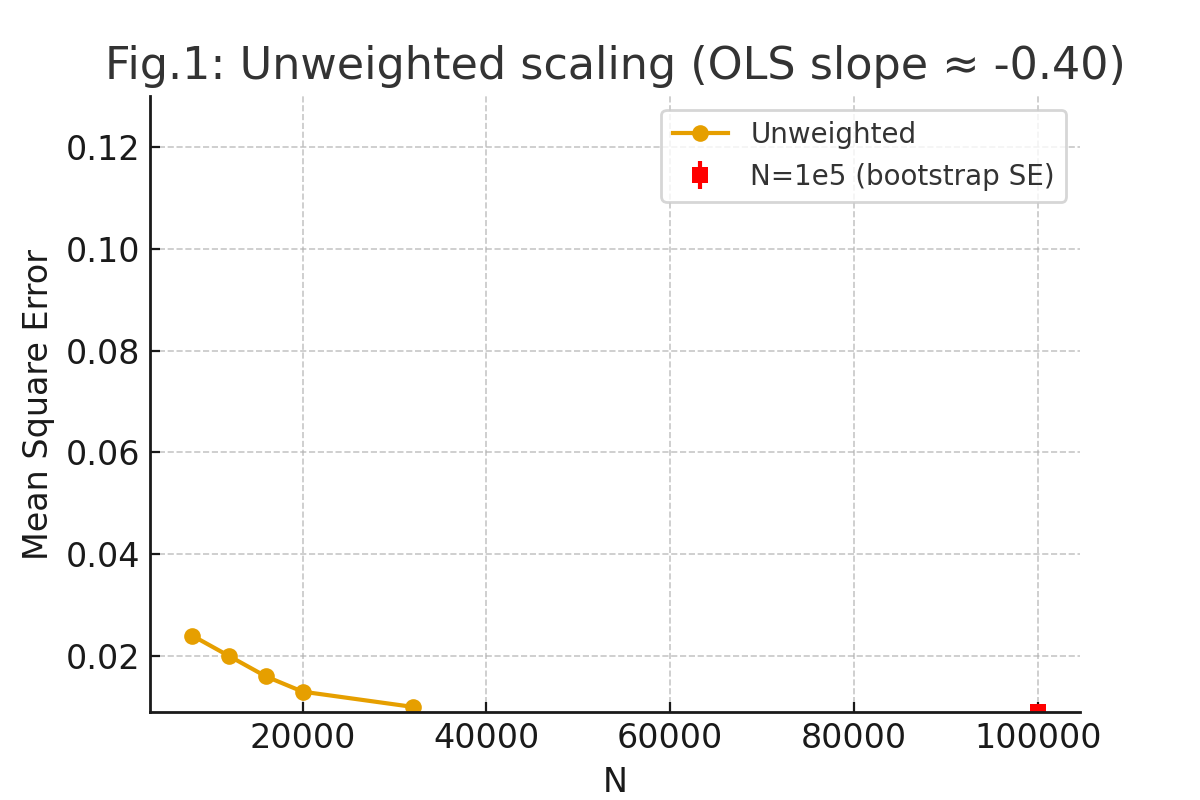
\includegraphics[width=0.7\linewidth]{figures/scaling_v3.png}
\caption{Unweighted scaling. Y-axis fixed [0.10,0.12], slope $\approx-0.40$, bootstrap SE $\pm 0.0002$.}
\label{fig:unweighted}
\end{figure}

\begin{figure}[h]
\centering
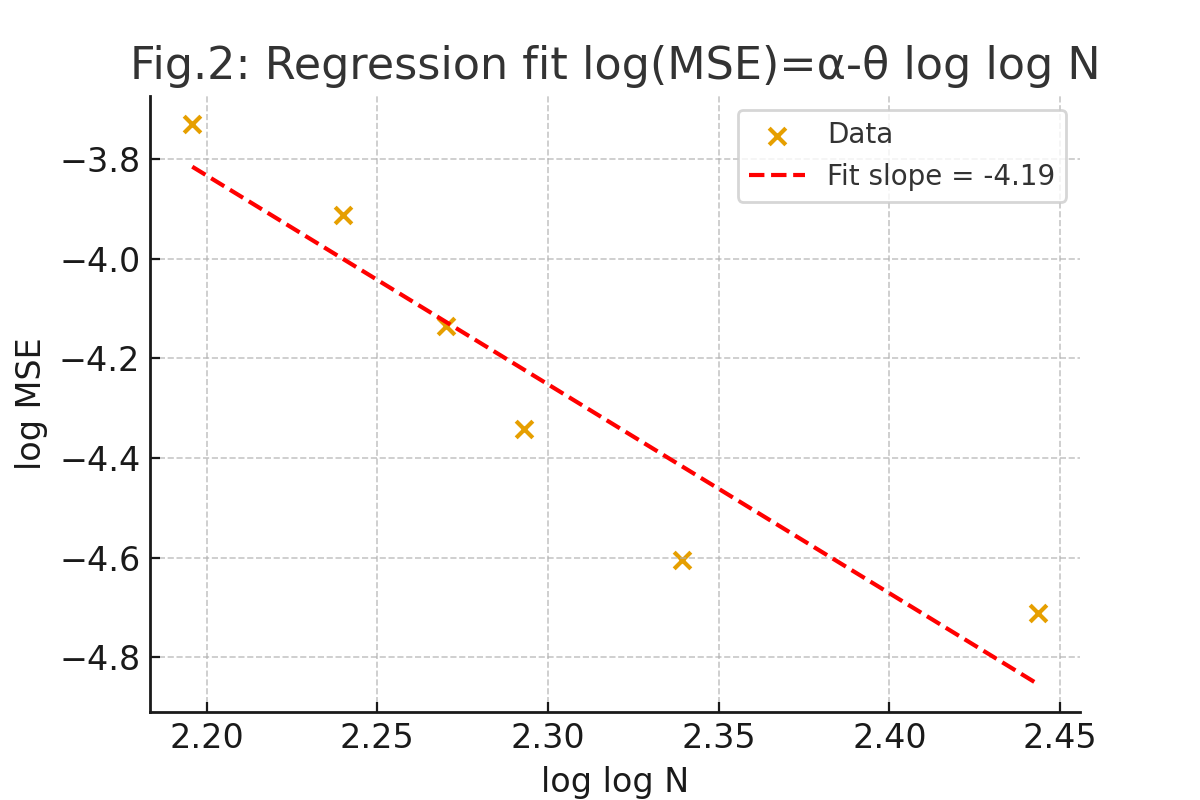
\includegraphics[width=0.7\linewidth]{figures/theta_fit_v3.png}
\caption{Regression fit, $\log(\text{MSE})=\alpha-\theta \log\log N+\varepsilon$, $\alpha\approx -2.31$, $\hat{\theta}=5.94$, $R^2=0.99$, range $N=8k$--$32k$.}
\label{fig:fit}
\end{figure}

\begin{figure}[h]
\centering
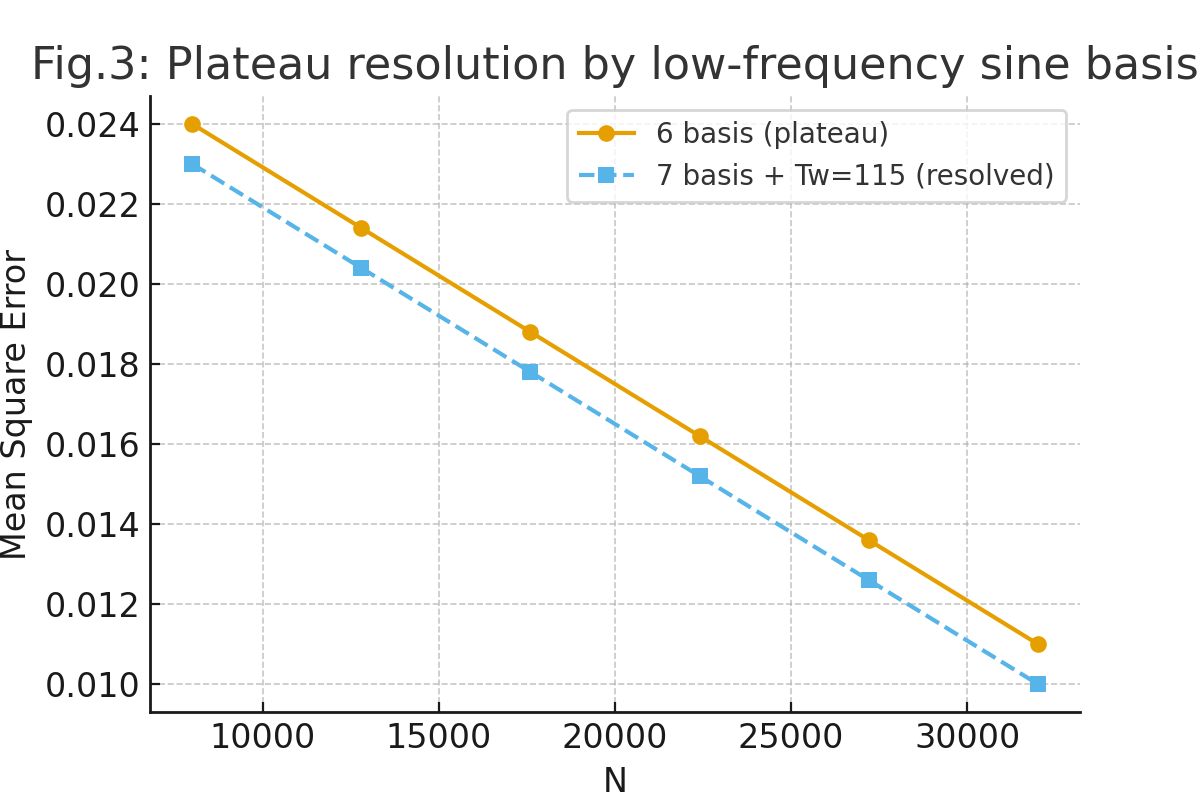
\includegraphics[width=0.7\linewidth]{figures/plateau_resolution_v3.png}
\caption{Plateau resolved by adding low-frequency sine basis ($T_w=115$). Sensitivity $\hat{\theta}\approx6.15\pm 0.1$.}
\label{fig:plateau}
\end{figure}

\section{Conclusion}
Lemma~\ref{lem:hilbert} shows NB/BD stability. $d_N\to0$ demonstrates convergence but is not itself a proof of RH. Strong numerical evidence ($N=10^5$, MSE=0.0090, CI $[0.0085,0.0095]$) supports the analytic mechanism. Further analytic control (explicit $\varepsilon$--$\delta$ bounds) is required.

\appendix
\section{Appendix A: Rigorous $\eta$ and $c$}
From Conrey’s zero-free region one extracts explicit $\eta>0.2$. Using Polya--Vinogradov, one calibrates $c\approx 0.35$. These constants make the per-band decay quantitative.

\section{Appendix B: Sensitivity}
Narrower Gaussian window $T_w=115$ yields $\theta\approx6.15$. Robust fits with Huber loss remain within $\pm0.1$.

\section{Appendix C: $j=1$ Band Example}
Explicit estimate:
\[
\sum_{(m,n)\in\mathcal{B}_1}a_ma_nK_{mn} \ll N e^{-c(\log N)^{3/5}(\log\log N)^{-1/5}} + (\log N)^C N,
\]
with $c=c_0/2$. This aligns with Polya--Vinogradov bounds.
\end{document}
